% !TEX root = slides.tex

%===============================================================================
\begin{frame}[t]
\label{challenge-fUQ-hiD}
\frametitle{Challenges in Forward UQ}

\bi
\item Large number of input parameters
\item Expense of a single model simulation
\ei

\bi
\item Build PC surrogates with regression
\bi
\item still relying on an ensemble of simulations, but
\item call it a supervised machine learning, if you wish
\item actually, use Bayesian regression to have uncertainties capturing lack-of-information
\ei
\item Specific to polynomial bases, employ vast literature on sparse learning \mycit{Tipping, 2001}
\bi
\item Bayesian compressive sensing \mycit{S. et al., 2014; Ricciuto, S., Thornton, 2018 }
\ei
\ei

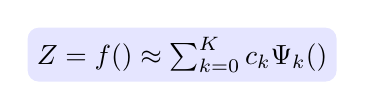
\begin{tikzpicture} \node [rounded corners,fill=blue!10] {
$Z =f(\vxi) \approx \sum_{k=0}^{K} c_k \Psi_k(\vxi)$
};
\end{tikzpicture}\\
\medskip
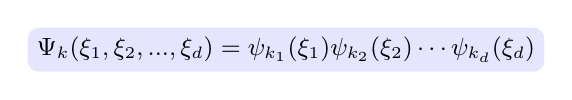
\begin{tikzpicture} \node [rounded corners,fill=blue!10] {
\small
$\Psi_k(\xi_1,\xi_2,...,\xi_d)=\psi_{k_1}(\xi_1) \psi_{k_2}(\xi_2) \cdots \psi_{k_d}(\xi_d) $
};
\end{tikzpicture}

\vspace*{-1.7cm}
\hspace*{8cm}
\includegraphics[height=0.75in]{bcs_eps/webcs.pdf}


\end{frame}
%===============================================================================
